\newpage
\section{Билет 1. Реляционная база данных. Область применимости и основные понятия. Отношение, атрибут, кортеж. Связь. Целостность данных.}

\textbf{Реляционные базы данных} представляют собой базы данных, которые используются для хранения и предоставления доступа к взаимосвязанным элементам информации. Вся информация изображена в виде простых таблиц, которые разбиты на строки и столбцы, на пересечении которых и расположена информация. Эта структура стала настоящим скачком вперед в развитии баз данных.

Реляционные БД находят применение повсеместно: В организациях для учёта персонала, ведения бухгалтерии, учёта товаров на складе, поставщиков, партнёров, клиентов, ведения электронного документооборота. В адресных и телефонных книгах, словарях, справочниках.

Таблицы называют \textbf{отношениями} (relations)— поэтому и базы данных называются реляционными. В терминах данной теории строки таблицы будут называться \textbf{кортежами}, а колонки — \textbf{атрибутами}.

\textbf{Связи между таблицами баз данных:}
\begin{itemize}
    \item \textit{связь один к одному} – самая редко встречаемая связь между таблицами. В 97 случаях из 100, если вы видите такую связь, вам необходимо объединить две таблицы в одну;
    \item \textit{связь один ко многим} реализуется тогда, когда объекту А может принадлежать или же соответствовать несколько объектов Б, но объекту Б может соответствовать только один объект А. Пример на Рис.\ref{fig:onekn};
    \item \textit{связь многие ко многим} реализуется в том случае, когда нескольким объектам из таблицы А может соответствовать несколько объектов из таблицы Б, и в тоже время нескольким объектам из таблицы Б соответствует несколько объектов из таблицы А. Пример на Рис.\ref{fig:nkn}
\end{itemize}

\begin{figure}[!h]
    \centering
    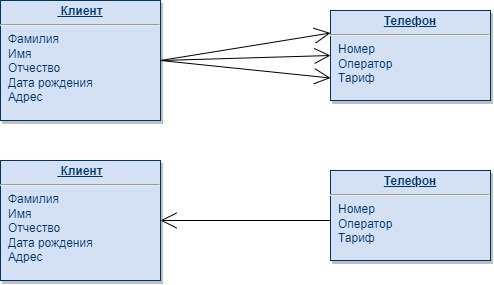
\includegraphics[scale = 0.5]{1/1kn.jpg}
    \caption{Связь один ко многим}
    \label{fig:onekn}
\end{figure}

\begin{figure}[!h]
    \centering
    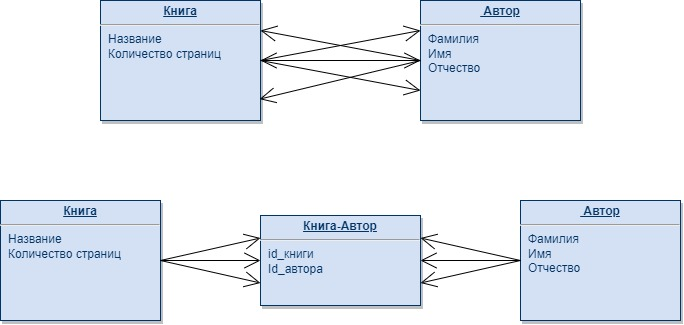
\includegraphics[scale = 0.5]{1/nkn.jpg}
    \caption{Связь многие ко многим}
    \label{fig:nkn}
\end{figure}


\textbf{Целостность данных:} 
Для пользователей важно, чтобы база данных отображала предметную область однозначно и непротиворечиво, т.е. чтобы она удовлетворяла условию целостности.

В теории баз данных под целостностью понимают свойство соответствия структуры и содержания базы данных предметной области. В реляционной модели данных определяются два основных требования, при которых обеспечивается целостность данных: \textbf{целостность сущностей} и \textbf{целостность ссылок.}

Каждый объект или наблюдение представляется в реляционной базе как группа взаимосвязанных элементов данных — кортеж некоторого отношения.

\textit{Требование целостности сущностей} заключается в том, чтобы каждый кортеж любого отношения отличался от другого кортежа этого отношения (т.е. любое отношение должно обладать первичным ключом).

\textit{Требование ссылочной целостности} состоит в том, что для каждого значения внешнего ключа, появляющегося в дочернем отношении, в родительском должен найтись кортеж с таким же значением первичного ключа.
